\chapter{Modeling}
\index{Modeling@\emph{Modeling}}%


\section{Overview}
To motivate the problem, we see both the literature a gap in looking at power grid repairs in a post-disaster context with consideration of the roads as well as specific identification of this problem from government agencies. The Federal Emergency Management Agency's 2017 post season after action report \cite{FEMA2017AAR} and Hurricane Sandy after action report \cite{FEMASandyAAR} identify the lack of coordination between agencies involved in recovery as a major shortcoming and call for increased coordination, particularly for the sake of recovery logistics.

We know from the earlier referenced literature that road repair is a concern in the wake of a hurricane. We assume for the sake of this thesis that all roads can be cleared of flooding and/or debris. Clearing here represents digging out drainage for minor flooding and clearing debris. Severely damaged roads should be treated as completely impassible and dropped from the graph representation of the network to allow this assumption to work in a practical context. While more severely damaged roads are eventually repaired, these repairs frequently represent involved construction efforts spanning weeks or months after a disaster and therefore are beyond the scope of the current modeling efforts.

We model the topology of both power and road networks as a pair of graphs with shared sets of nodes. On the road graph, the nodes are the physical locations of power substations and buses. We abstract away from the roads to a representation of them that captures effects of the road grid existing, but simplifies routing. A more full representation of the road network would include dummy nodes into the road network to represent major intersections, letting the edges/roads represent the shortest paths between those points. This typically comes at the cost of a dramatic increase in runtime as routing-based problems are computationally intense. Therefore we elect to use an abstracted representation based on existing literature on road grid modeling \cite{ChanEA2011} that treats a road network as an abstraction based on frequently traveled paths. 

The nodes representing power substations, generators, and/or buses are mirrored on the power network layer, but the edges at this layer represent the power line connections between substations. This multilayered graph depiction of the two infrastructures allows cleaner mathematical modeling later on. With a given post-disaster damage to both networks (damaged nodes and lines in the power grid and damaged roads in the road network), we analyze of the interactions in the repair efforts needed to get both networks fully operational.

We model time in discrete shifts because it allows for mixed-integer programming to solve both problems in a way where their solutions can be temporally aligned. This temporal alignment allows for interaction frameworks to remain simple.

We assume that direct current (DC) approximations of power flow can accurately approximate the full alternating current (AC) power flow of a real power grid. DC power flow is more accurate than a ``pipe-flow" representation as it captures some of the physics behind electrical flows. This interaction may be important in the consideration of repair and resilience. DC power flow models spread flow out among possible lines whereas pipe-flow style models load all the demand onto single lines due to how they are solved with linear programming since those methods will seek an extreme point solution. DC representation is usually within 5-10\% of the AC power flow solutions \cite{Frank2016} \cite{StottEA2009} making it appropriate for the power repair problem. Since we are considering is one of logistics and not one of power flow management, an approximation of the power flow that relaxes numerical accuracy of power flow but leaves a near optimal repair schedule is justified. We model only the power demand in terms of wattage and not voltage because voltage sag disruptions are a problem primarily at the distribution level \cite{LamoreeEA1994}. Additionally, keeping voltage inside the desired range is a problem of optimal grid control, which is not considered in this thesis \cite{MiretEA2013}.  

With the power grid, we treat distribution below the substation level as a point load associated with a substation. Each substation in real power grid has a distribution level network that services the local area by connecting individual demand such as a house to the power grid as a whole. The wires between substations are considered the transmission level network. The choice to discard the distribution network's topology in the modeling of repair scheduling stems from two factors. First, the distribution network stemming from a substation has geographically co-located damage as distribution areas from a single substation are geographically compact. This implies that including road networks with distribution grid repairs would provide little benefit, as time costs from transiting between one damaged element and another are small. Secondly, flow at the distribution level goes from the substation to the demand sites unlike transmission level networks where flow can go in different directions depending on the state of the grid. This is different from operation of transmission level networks so they can be treated as a point load on the transmission network, avoiding complexity that does not improve insights about the core interaction of concern.

\section{Direct Current Optimal Power Flow (DC-OPF)}
To model repair of damaged power grids, we first must understand the Direct Current-Optimal Power Flow (DC-OPF) model as it forms the basis of all of the more complex power models used in this thesis. The problem can be expressed as satisfying all power demand at minimal generation cost--a problem that shows up frequently in control and analysis of power grids. The power grid can be represented as a graph with edges representing power lines and the nodes of the directed graph corresponding to substations and buses. These substations may service a distribution area with associated unmodeled distribution network. Directionality in the graph is done for bookkeeping as power can flow both directions and by having the graph be directed, we can allow positive flow on edge $(i,j)$ to represent power flow going from $i$ to $j$ and negative flow representing power going from $j$ to $i$. This leads to the nodes representing buses and substations having edges that connect the nodes indexed from lower to higher. For example, edge $(1,2)$ would be included in this modeling, edge $(2,1)$ would not be as it would just be represented as negative flow on edge $(1,2)$.


We use the following notation for clarity in models:
\begin{itemize}
	\item $o(e)$ is the node at the origin of line $e$ 
	\item $d(e)$ is the node at the destination of line $e$
	\item $O(i)$ is the set of lines with origin $i$
	\item $D(i)$ is the set of lines with destination $i$
\end{itemize}
We define the following parameters and sets:
\begin{itemize}
	\item $N$ is the set of nodes indexed by $i$
	\item $E$ is the set of edges indexed by $e$
	\item $C_i$ is the cost of producing one unit (megawatts in this thesis) of power at node $i$
	\item $P_i$ is the maximum power generation in megawatts for node $i$. If there is no generator connected to the substation, maximum production is zero watts.
	\item $D_i$ is the demand for power in megawatts at node $i$
	\item $B_e$ is the line susceptance in per unit siemens for power line $e$ (susceptance is the measure of ease of power flowing along a line)
	\item $\overline{L_e}$ is the maximum amount of flow in megawatts on line $e$
	
\end{itemize}
We also have the following decision variables:
\begin{itemize}
	\item $X_e$ is the power flow on line $e$ 
	\item $Y_i$ is the power generated at node $i$ in megawatts
	\item $\theta_i$ is the phase angle in radians for power flow at node $i$ 
\end{itemize}
The model can then be formulated as follows: 
\begin{equation}
\textnormal{Minimize} \sum_{i\in N} C_i Y_i
\end{equation} 
subject to
\begin{eqnarray}
X_e = B_e (\theta_{o(e)} - \theta_{d(e)}), \hspace{4pt} \forall e \in E\\
Y_i - \sum_{e \in O(i)} X_e + \sum_{e \in D(i)} X_e = D_i, \hspace{4pt} \hspace{4pt} \forall i \in N\\
Y_i \leq P_{i}, \hspace{4pt} \hspace{4pt} \forall i \in N	\\ 
-\overline{L_e} \leq X_e \leq \overline{L_e}, \hspace{4pt} \forall e \in E\\
Y_i \geq 0, \hspace{4pt} \forall i \in N\\
-\pi/2 \leq \theta_i \leq \pi/2, \hspace{4pt} \forall i \in N.
\end{eqnarray}

To explain, the problem is generation power at the minimum cost in a way that satisfies all of the demand subject to the physics of how DC-approximated power grids operate. This problem also solves out line flow amounts and phase angles for each node as expressed in a per unit basis (normalizing everything to the same basis unit such as megawatt). Constraints (2.2) are part of the DC approximation to AC power flow where we assume sin($x$) = $x$ for small values of $x$ and reduce power flow to just its real component (dropping the reactive component of power flow). This representation of power flow tracks only power demand (wattage) and neglects voltage as it is less relevant to this problem, but both versions of DCOPF are a well solved problems in electrical engineering literature \cite{Frank2016} \cite{EldridgeEA2017} \cite{ZhangChow2015}. Constraints (2.3) are a set of standard flow balance constraints that require power going into a node has to be equal to power coming out of node. Constraints (2.4) restrict power generation to the maximum permitted for the generator. Constraints (2.5) model flow capacity for power lines. Constraints (2.6) impose non-negativity limits on generation and constraints (2.7) limit the phase angle to a single period of the sine wave. While overall a simple problem, DCOPF serves as the building block for most of the power grid models used for the rest of this thesis as well as being used in practice for controlling power grid generation and dispatch \cite{LiBo2007}. 
\section{Validating Use of DC Power Flow}

Much of the existing literature in operations research relaxes one step further than DC powerflow all the way to traditional network flow or ``pipe-flow" models that can be used for any abstracted network. For these problems, DC powerflow models are sometimes considered to be unnecessary. This therefore begs the question of why use it over a traditional network flow model. We define traditional network flow to consist of just flow balance and line limits (analogous to relaxation of constraint (2.2) in the DCOPF model below). DC power flow tends to spread power flow out more across lines due to the physics of power flow in a grid while a simpler network flow model tends to seek an extreme point solution, leading to fewer lines under use with heavier loading on those lines as a byproduct of solving it with a linear program. To demonstrate this effect, we solve DCOPF and its corresponding relaxation of constraint (2.2) on IEEE 30 bus and IEEE 57 bus. The results shown in Figure 2.1 show a small but noticeable difference in flow patterns. This may be relevant when modeling system-wide damage in a power grid. Therefore it is worth including in models for repair and resilience. In addition to this, the computational cost of including DC power flow over a pipe-flow model is near zero because extra linear variables have a low impact on runtime of branch-and-bound based solvers. Additionally, this modeling change helps keep math representation of the network closer to the real AC flow, which has the added benefit of making it easier to persuade practitioners in the field that the models presented using DC power flow have relevance to real operations.

\begin{figure}
	\centering
	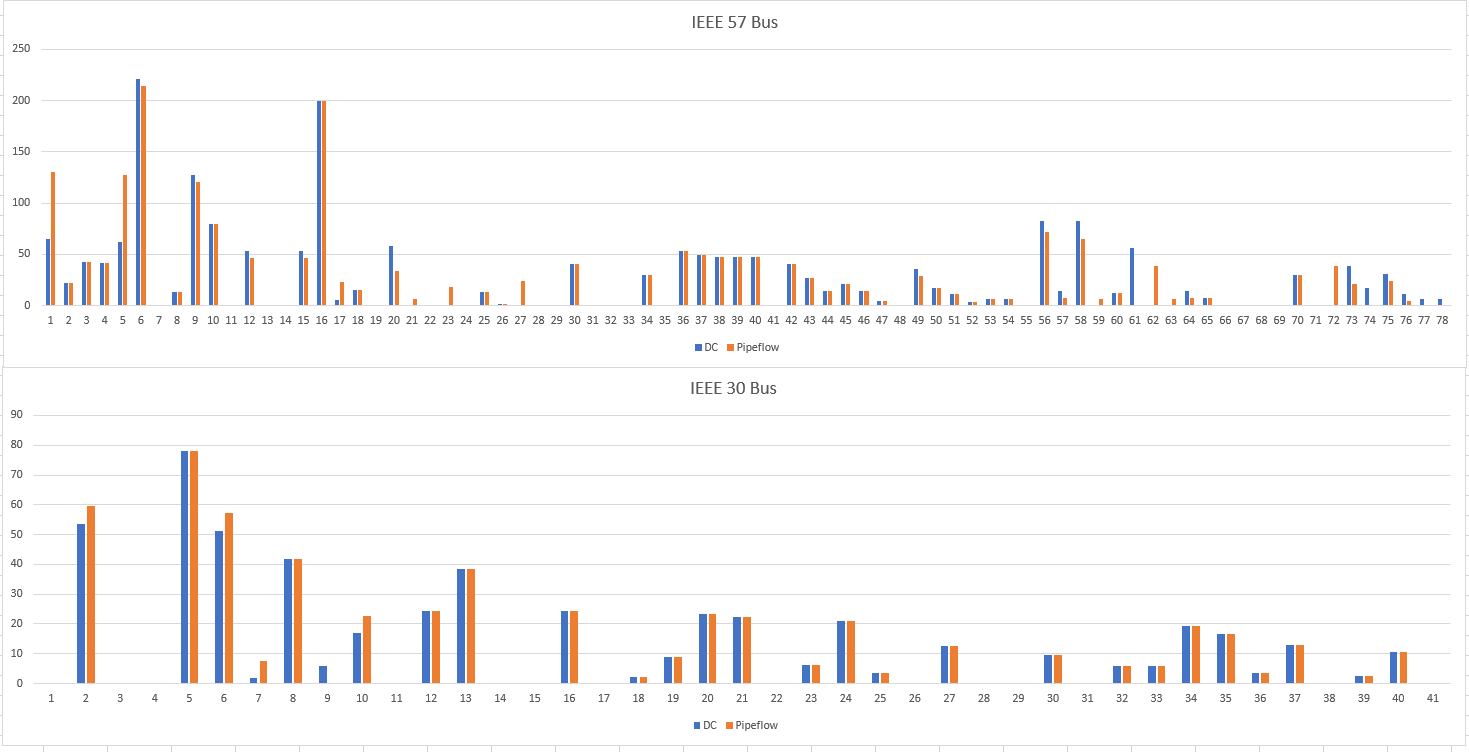
\includegraphics[width=\linewidth]{DCvsPipeflow.PNG}
	\caption{Comparison of DC and traditional (pipeflow) network flow}
\end{figure}

Further, as we extend this model to resilience, use of pipeflow style network models to handle power flow may over-prioritize the resilience of certain lines which strays from optimality on the full AC power grid. Since DC power flow is of low computational cost and low model complexity to add and has upside in some limited cases, we find its inclusion to be warranted.

\section{Road Repair Problem}
When dealing with repairs on the power grid, we need a framework for solving problems based on the damage to the road network. Any framework will rely on a method for modeling repair of the road network. We elect to solve the road repair problem as a scheduling/routing problem for a crew tasked with clearing debris and/or digging out minor flooding, following Duque et al. \cite{DuqueEA2016} and their treatment of how road repairs function. This takes the form of using routing the crew down a damaged road at higher time cost. This is solved by constructing a series of roads to traverse as a tour that begins and ends at a depot in every shift. We model this as follows:

\textbf{Parameters and Sets:}
\begin{itemize}

\item $T$ is the set of time periods (shifts) over the time horizon, indexed by $t$
\item $N$ is the set of nodes in the graph with node 1 being the depot, representing the locations of substations where each substation could have a distribution load, a generator, or both
\item $c_{ij}^t$ is the measure of the value of the road segment from node $i$ to node $j$ during period $t$. $i,j$ pairs that do not have a road between them have value zero.
\item $l_{ij}$ is the transit time in hours of the road segment between nodes $i$ and $j$ under nominal conditions
\item $r_{ij}$ is the time to repair the road segment between nodes $i$ and $j$ (hours), $r_{ij}$>$l_{ij}$ $\forall i,j$ since lines are repaired by transiting them
\item $s^t$ is the length of shift period $t$ in time units (hours)
\item $o_{ij}$ is the initial condition (1 is working, 0 is not) of the road segment between nodes $i$ and $j$
\end{itemize}

\textbf{Decision Variables:}
\begin{itemize}
\item $X_{ij}^t$ is the binary variable for road segment $ij$ being operational in time $t$
\item $Y_{ij}^t$ is the binary variable for travel from $i$ to $j$ being in the tour at time $t$
\item $W_{ij}^t$ is the length of travel time for road segment $ij$ at time $t$
\end{itemize}

Given the parameters and decision variables, we formulate the model as follows:
\begin{equation}
\textnormal{Minimize} \sum_{t \in T}  \sum_{i,j \in N} c_{ij}^t(1-X_{ij}^t) 
\end{equation}
subject to:
\begin{eqnarray}
\sum_{j \in N} Y_{1j}^t = 1,\hspace{6pt} \hspace{6pt} \forall t\in T \\
\sum_{i,j \in N} W_{ij}^t Y_{ij}^t \leq s^t, \hspace{6pt} \forall t\in T \\
W_{ij}^t = \max \{l_{ij}, r_{ij}(1-X_{ij}^t) \}, \hspace{6pt} \forall t\in T, \hspace{5pt} \forall i,j \in N\\
\sum_{j \in N} Y_{ij}^t - \sum_{j \in N} Y_{ji}^t = 0, \hspace{6pt} \forall t\in T, \hspace{5pt} \forall i \in N\\
X_{ij}^t \le \sum_{t'=0}^{t-1} Y_{ij}^{t'} + o_{ij} , \hspace{6pt} \forall t\in \{1,2,....t_{max}\},  \hspace{5pt} \forall i,j \in N\\
\sum_{i,j \in S; i\neq j} Y_{ij}^t \leq |S|-1, \hspace{6pt} \forall S \subset N, \hspace{2pt} S \neq \emptyset, \hspace{5pt} \forall t\in T\\
W_{ij}^t \geq 0, \hspace{5pt} \forall t\in T, \hspace{5pt} \forall i,j \in N \\
X_{ij}^t,Y_{ij}^t, \in \{0,1\}. 
\end{eqnarray}

To explain the modeling, the objective is to minimize the value of out-of-service road. Value here is defined loosely so that without loss of generality, this can be substituted with a set of priority weights from another agency that cares about the road network's operation. For example, the value metric for the road network can be selected based on an agency such as the Red Cross or FEMA that is tasked with bringing relief supplies in to a disaster-stricken area. This modeling is done to capture the issue of both power and road utilities having different priorities when it comes to restoring infrastructure.

Constraints (2.9) force the depot to be in every tour. Constraints (2.10) provide a scheduling constraints that limit the tour's length to the length of the shift. Constraints (2.11) are nonlinear but linearizable constraints that set the length of a road to either its nominal operation time or its repair time depending on whether or not it is marked as working ($X_{ij}^t$ = 1). Constraints (2.12) are standard path connectivity constraints. Constraints (2.13) restrict each road segment to only be working if it started working ($o_{ij}$ = 1) or has been repaired. Constraints (2.14) are a standard set of subtour elimination constraints. Constraints (2.15) and (2.16) exist to restrict decision variables to only valid values.

Of note is that constraints (2.10) and (2.11) are nonlinear as intuitively expressed. We linearize it by rewriting constraints (2.10) and (2.11) as the following:

\begin{eqnarray}
\sum_{i,j \in N} W_{ij}^t \leq s^t, \hspace{6pt} \forall t\in T \\
W_{ij}^t \leq MY_{ij}^t, \hspace{6pt} \forall t\in T, \hspace{5pt} \forall i,j \in N\\
W_{ij}^t \geq l_{ij}Y_{ij}^t, \hspace{6pt} \forall t\in T, \hspace{5pt} \forall i,j \in N\\
W_{ij}^t \geq (1-X_{ij}^t)r_{ij} - (1-Y_{ij}^t)M, \hspace{6pt} \forall t\in T, \hspace{5pt} \forall i,j \in N.
\end{eqnarray}


\section{Power Grid Repair Problem}
When looking at repair of the power grid at the transmission level, we formulate a discrete time mixed integer program that captures both the planning/scheduling/movement of repair crews as well as the DC power flow model. We assume the following:
\begin{itemize}
	\item Repair of a power line can be started from either end of that power line.
	\item Minimum spanning tree's lower bound on the length of a tour/route provides a usable approximation for the sake of keeping model runtime down 
	\item Load shedding can be modeled as a continuous loss even though on real power grids it is a series of discrete decisions to stop power to specific parts of the distribution network that allows for small increments of load to be shed, though not truly continuous power shedding. We make this assumption due the the modeling and computational burden of having many low-impact decisions to make.
	\item Every substation can have an associated demand from an attached distribution network as well as generation capacity from an attached power plant. For substations that do not have these attached, the node demand and/or power generation capacity are set to 0.
\end{itemize}
We pose the model as follows:
\newline
\textbf{Sets and indices:}
\begin{displaymath}
\begin{array}{ll}
N & \mbox{set of nodes, indexed by $i$} \\
E & \mbox{set of power lines, indexed by $e$}\\
R & \mbox{the set of road segments} \\
T & \mbox{the planning horizon, indexed by $t$}  \\
O(i) & \mbox{set of lines with origin $i$} \\
D(i) & \mbox{set of lines with destination $i$} \\
o(e) & \mbox{origin node of line $e$} \\
d(e) & \mbox{destination node of line $e$} \\
\end{array}
\end{displaymath}
\textbf{Parameters:}
\begin{displaymath}
\begin{array}{ll}
\overline{L_e} & \mbox{maximum power flow for line $e$ in terms of megawatts}\\
R_{i} & \mbox{time to repair node $i$ in hours} \\
R_{e} & \mbox{time to repair line $e$ in hours}\\
C_{ij}^t & \mbox{length of the shortest path from node $i$ to node $j$ at time $t$}\\
D_i & \mbox{power demand in megawatts at node $i$ in the pre-disaster state}\\
P_k & \mbox{maximum power generation in megawatts for generator $k$}\\
B_e&  \mbox{line susceptance in siemens per unit for power line $e$}\\
I_e, I_i & \mbox{binary initial condition of line $e$ and node $i$, respectively (1 is operational)}\\
F & \mbox{Maximum length of shift in hours}
\end{array}
\end{displaymath}
\textbf{Decision Variables:}
\begin{displaymath}
\begin{array}{ll}
X_{e}^{t} & \mbox{power flow in megawatts on line  $e$ at time $t$}\\
G_{k}^t & \mbox{production from generator $k$ at time $t$}\\
Y_{n}^t & \mbox{load shed from bus $n$ at time $t$}\\ 
V_i^t & \mbox{binary variable for node $i$ being operational at time $t$ (1 is operational)}\\
W_{e}^t & \mbox{binary variable for line $e$ being operational at time $t$ (1 is operational)}\\
U_{e}^t & \mbox{binary variable for line $e$ serviced at time $t$}\\
Z_i^t & \mbox{binary variable for node $i$ serviced at time $t$}\\
\theta_i^t & \mbox{phase angle in radians for the power flow at $i$ in time $t$}\\
M^t & \mbox{length of the tree used for ``routing'' at time $t$ measured in hours} \\
Q_{ij}^t & \mbox{indicator for $ij$ being in the spanning tree at $t$}
\end{array}
\end{displaymath}

Given these parameters and decision variables, we format the model as follows:
\begin{equation}
\textnormal{Minimize} \sum_{i \in N} \sum_{t \in T} Y_{it}
\end{equation}
subject to:
\begin{eqnarray}
X_e^t = B_e (\theta_{o(e)}^t - \theta_{d(e)}^t), \hspace{5pt} \forall t \in T, \hspace{4pt} \forall e \in E\\
G_i^t - \sum_{e \in O(i)} X_e^t + \sum_{e \in D(i)} X_e^t = D_i-Y_i^t, \hspace{4pt} \forall t \in T, \hspace{4pt} \forall i \in N\\
0\leq G_k^t \leq P_{k} V_{k}^t, \hspace{4pt} \forall t \in T, \hspace{4pt} \forall k \in N\\
0\leq Y_i^t \leq D_i, \hspace{4pt} \forall t \in T, \hspace{4pt} \forall i \in N\\
-\overline{L_e}W_{e}^t \leq X_{e}^t \leq \overline{L_e}W_{e}^t, \hspace{4pt} \forall t \in T, \hspace{4pt} \forall e \in E\\
-\overline{L_e}V_{o(e)}^t \leq X_{e}^t \leq \overline{L_e}V_{o(e)}^t, \hspace{4pt} \forall t \in T, \hspace{4pt} \forall e \in E\\
-\overline{L_e}V_{d(e)}^t \leq X_{e}^t \leq \overline{L_e}V_{d(e)}^t, \hspace{4pt} \forall t \in T, \hspace{4pt} \forall e \in E\\
V_i^t \leq \sum_{t'=0}^{t-1} Z_i^{t'}+I_i, \hspace{4pt} \forall i \in N, \hspace{4pt} \forall t\in \{1,2,....t_{max}\}\\
W_{e}^t \leq \sum_{t'=0}^{t-1} U_{e}^{t'}+I_e,\hspace{4pt} \forall t\in \{1,2,....t_{max}\} \hspace{4pt} \forall e \in E\\
M^t = \sum_{i \in N} \sum_{j \in N} C_{ij}^t Q_{ij}^{t},  \hspace{4pt} \forall t \in T\\
\sum_{i \in N} \sum_{j \in N} Q_{ij}^{t} = \sum_{i \in N} Z_i^t + \sum_{e \in E} U_e^t - \sum_{i \in N} Z_i^t \sum_{e \in O(i) \cup D(i)} U_e^t, \hspace{6pt} \forall t \in T\\
\sum_{i,j \in S} Q_{ij}^t \leq |S|-1, \hspace{6pt} \forall S \subset N, \hspace{2pt} S \neq \emptyset, \hspace{5pt} \forall t\in T \\
\sum_{j \in N} Q_{ij}^t \leq Z_i^t + \sum_{e \in O(i) \cup D(i)} U_{e}^t, \hspace{6pt} \forall t \in T, \hspace{4pt} \forall i \in N \\
\sum_{e \in E} R_{e}U_e^t + \sum_{i \in N}R_{i}Z_i^t + M^t \leq F, \hspace{6pt} \forall t \in T\\
Q_{ij}^t,U_{e}^t,Z_{i}^t,W_{e}^t,V_{i}^t \in \{0,1\}. 
\end{eqnarray}

The objective here is to minimize the amount of load shedding (failure to service demand) where zero load shed would represent nominal operation of the power grid. This is equivalent to maximizing the amount of demand satisfied over the repair horizon. Constraints (2.22) are in place to handle line susceptance and phase angle related power flow. Constraints (2.23) are the flow balance constraints from DCOPF with the change that demand can not be satisfied ("shed") at penalty to the objective function. Constraints (2.24) are a generation capacity constraint set where generation of power can only flow into the grid if the bus that the generator connects to is intact. Constraints (2.25) handle amount of load shedding at each bus so that the maximum load shed is 100\% of the demand. Constraints (2.26-2.28) are flow limit constraints subject to functioning of the line and buses on both sides of the corresponding line. Constraints (2.29) and (2.30) regulate the functionality of a power grid element so that an element can only be operational ($V_i^t$ or $W_e^t$ = 1) if it started operational or was repaired before the current shift. These are inequality constraints rather than equality constraints to allow elements to be switched off if that decision would allow more power demand to be satisfied.

Constraints (2.31) define the length of a minimum spanning tree based on elements selected to be repaired. This is done for readability reasons, since there is no reason that it can not be folded into (2.35). Constraints (2.32) are a quadratic constraint set that counts how many elements need to be inserted into the minimum spanning tree using inclusion/exclusion counting to handle repairs where a bus and a line that connects to the bus both get repaired. Unlike other quadratic constraints in this thesis, this one is not linearized. As the quadratic term is of the form of multiplying two binary decision variables, Gurobi is able to solve these constraints directly. As we are modeling under the assumption that a line's repair can start from either endpoint, we need to account for the cases where a bus and its attached node are repaired in the same shift when planning the spanning tree approximation to the route. Constraints (2.33) are standard subtree elimination constraints. Constraints (2.34) restrict the inclusion of elements in the tree to only nodes that are repaired or are the site of a line repair. While a route could go through other nodes, we compute the shortest paths between nodes to keep the minimum spanning tree as simple as possible. Constraints (2.35) are scheduling constraints that matches the ones seen in the road repair model to restrict the total operations in each shift to the length of the shift. We note that this model does not fully generate the route and it would have to be constructed as a post processing step to solve the actual route. Routing problems for a given set of elements are well-studied as well as computationally easy on this scale. Given that the route cost is approximated, this problem remains feasible 




\section{Lower Bounding and Post Processing Heuristic}

From the previously presented models, we recognize that we can generate a lower bound using these models. While the MST method provides a lower bound on a routed solution, by not considering travel times at all, we find a lower bound on any repair procedure that can be planned. By setting all the travel times to zero (${C}_{ij} = 0$), leaving the rest of the model in place, we provide a lower bound as it generates an optimal repair schedule ($K_{lb}^t$) that is compressed into the minimum possible time. This can then be post processed into a feasible schedule ($K_{h}^t$) by starting with the lower bound schedule and then repacking it into shifts using the following algorithm to generate a heuristic solution to the repair problem:

\begin{enumerate}
	\item create a feasible list ($F$) that will be used to track repairs that can be put into the post processed schedule, a priority list ($P$) of repairs that have been on the feasible list before, an index ($I$) to track what shifts are in the search, $S$ as the current shift of repairs, and a tracker of the current node ($N$).
	\item Begin by assigning $I=1$ .
	\item Move any repairs remaining on $F$ to $P$
	\item Move any repair from $K_{lb}^t$ in shift $I$ to $F$
	\item Set $N$ to the pre-defined depot location for repairs
	\item Calculate the time to reach and repair every item in both $P$ and $F$ from $N$. For edge repairs, choose the endpoint of the edge with lower cost for travel and repair.
	\item If there are unassigned node repairs in $P$ that can be added to $S$ without having the time cost of $S$ exceed the allowed length of a shift, assign the lowest cost node repair to $S$. Set $N$ to be the site of repair. Return to step 6 
	\item If there are unassigned edge repairs in $P$ that can be added to $S$ without having the time cost of $S$ exceed the allowed length of a shift, assign the lowest cost edge repair to $S$. Set $N$ to be the site of repair. Return to step 6.
	\item If there are unassigned node repairs in $F$ that can be added to $S$ without having the time cost of $S$ exceed the allowed length of a shift, assign the lowest cost node repair to $S$. Set $N$ to be the site of repair. Return to step 6.
	\item If there are unassigned edge repairs in $F$ that can be added to $S$ without having the time cost of $S$ exceed the allowed length of a shift, assign the lowest cost edge repair to $S$. Set $N$ to be the site of repair. Return to step 6. 
	\item If there are no repairs that can be added to $S$, set shift $I$ in $K_h^t$ to be $S$. 
	\item $I$ = $I+1$
	\item Once every repair from the $K_{lb}^t$ has been assigned to a shift, end the algorithm.
\end{enumerate}

This is  similar to many greedy heuristics for knapsack problems where the lowest cost element is added to the knapsack. This method leverages the knowledge of what order repairs occur in the lower bound schedule to quickly add in the impact of travel time. This heuristic runs in polynomial time for the post processing. The  mixed integer program to generate the lower bound schedule is non-polynomial by virtue of being a mixed integer program though it runs in under a minute for both IEEE 30 bus and IEEE 57 bus power girds. As we show later, this process yields solutions that are close to our full model solutions across a variety of example cases. The reason to use this heuristic is that it allows for scheduling models for repairs to grow more complex while presenting a method for incorporating travel times after solving the optimal schedule.

\section{Road Power Interaction Frameworks}
Now that we have established both models that will be used to draw insights from the repair problem, we now outline how we handle their interactions. Since the models are solved independently, we have to choose one of them to be the first mover and the other to be the second mover. We therefore lay out the following frameworks:
\begin{itemize}
	\item \textbf{Road First}-- We model the problem as if the road grid decision maker has priority over the power grid decision maker in the combined repair effort. This is done by solving the road model, then treating the road model repair schedule as an input to the power model as a time-varying shortest path matrix.
	\item \textbf{Power First} -- We model the problem with the power grid as the first mover by solving the power grid repair problem with the roads at their nominal lengths. Presume that due to coordination effects, road segments are repaired before they are needed in the power grid repair schedule. To account for this delay while waiting for road repair, we introduce a one shift delay before the start of power repairs, assuming that one shift is enough for road repairs needed by the power grid.
	\item \textbf{Uncoordinated Repairs} -- To handle the case where the power grid decision maker may have to commence repairs with no prior information about the repair plan for the roads, but they have an assessment of the state of the roads in the wake of a hurricane. We model the roads as if they are damaged and their state does not change. Travel times for a damaged road segment are significantly longer due to debris and/or flooding, so longer alternate routes are usually used.
	\item \textbf{Heuristic} -- Using the heuristic described above, we can take the lower bound schedule constructed without travel times. These solutions are farther from the lower bound than solutions based on interacting the full models, but they are computationally fast and can be used to quickly gain insight about the repair problem to direct future plans.
\end{itemize}

